\chapter{O CERN e Física Experimental de Altas Energias}

O CERN ({\it Centre Européene pour la Rechèrche Nucleaire}) é o maior
laboratório de Física de Partículas do mundo, situado na fronteira da Suíça com
a França, contando com a colaboração de cientistas vindos de institutos
do mundo todo. Desde sua fundação em 1954, tem sido uma das referências de
avanços tecnológicos. Dentre seus feitos constam a construção do primeiro 
colisionador de prótons-prótons (1971), a descoberta 
da corrente de neutrons (1973), dos bóssom Z e W (1983), 
e a invenção da Web (1990) \cite{webCERN}. O acelerador de partículas mais ambicioso 
\cite{Intro_Standard} já construido é o \emph{Large Hadron
Collider}, o atual experimento do CERN, onde espera-se que o maior de seus 
detectores, o ATLAS, dê respostas a diversas questões da Física de Partículas
Elementares e da natureza do universo.

Este trabalho está inserido no ambiente de colaboração internacional do detector
ATLAS. O propósito deste capítulo é descrever a base para o entendimento desse ambiente
e os ferramentais nele utilizados. Serão introduzidos o estudo de Física de Partículas
Elementares e o Modelo Padrão (seção \ref{sec:fis_part}), 
o experimento LHC (seção~\ref{sec:lhc}), o detector
ATLAS (seção~\ref{sec:ATLAS}), dando enfoque ao seu sistema de calorimetria
(seção~\ref{ssec:calorimetria}), assim como o ferramental utilizado pela colaboração
(seção~\ref{sec:ferramentas}).

\section{Introdução a Física das Partículas Elementares}
\label{sec:fis_part}

Se dá o nome de Física de Partículas Elementares ao estudo dos contituintes
elementares e da natureza do universo. Embora a noção de que a matéria é
composta por um conjunto de constituintes elementares tenha surgido em cerca de
430 a.C., por Demócritos \cite{democritos}, o seu estudo na ciência moderna teve ínicio apenas 
no século 19, quando o elétron foi descoberto por Thompson \cite{thompson}.
Uma das grandes conquistas do século 20 foi o desenvolvimento do Modelo Padrão
de Física de Partículas Elementares.  

Qualquer teoria de Física de Partículas Elementares precisa ser consistente com
a Relatividade Especial. A junção da Mecânica Quântica, Eletromagnetismo e
Relativaidade Especial foi realizada através da Lei de Dirac e da Teoria de
Campo Quântico. A Teoria de Campo Quântico teve como seu primeiro triumfo a
Eletrodinâmica Quântica (QED), que descreve a interação de elétrons com o campo
eletromagnético. 

O Modelo Padrão, como o QED nele contido, é uma teoria de
interação de campos. A construção do Modelo Padrão foi guiada pelos principios 
de simetria, que podem ser divididos em diversos grupos com diferentes
propriedades matemáticas. A conexão entre a física e simetria é forte, como
demonstrado pelo teorema de Noether, onde essencialmente, para cada simetria
continua na natureza existe uma lei de conversação correspondente, podendo ser
citado a pressuposição da homogeniedade do espaço-tempo, o que leva ao lagrangiano
invariante para translações uniformes no espaço-tempo e, finalmente, a
transformações simétricas no sistema, tendo como consequência a lei da conservação 
de massa e momento \cite{Intro_Standard}. 

O Modelo Padrão descreve de maneira bem sucedida as relações entre
partículas elementares conhecidas pela ciência atual 
\cite{Intro_Nuclear} e as características de
três forças que interagem com essas partículas:
eletrogmagnetismo, forças fracas e forças fortes. A força gravitacional é
desprezível na escala da Física de Partículas, onde a massa da partículas é da
ordem de $10^{-27}$ kg \cite{Intro_Standard}.

As unidades normalmente utilizadas no estudo de Física de Partículas são fm para
distância (equivalente a $10^{-15}$ m), MeV ou GeV para massa ou energia, onde 1
eV (elétron-Volt) é a energia necessária para aumentar o potêncial elétrico de
um elétron em um volt, equivalente a $1,6\times10^{-19}$ J no SI, ou em unidades
de massa 1eV/$c^2$ = $1,78\times10^{-36}$ kg. A unidade para
área é o \emph{barn}, definida por 1 b = $10^{-28} m^2$, utilizada em
termos de mb ou fb \cite{Intro_Nuclear}.

O Modelo Padrão utiliza doze férmions, partículas elementares, divididas em dois grupos: os
léptons e os quarks. Existem três diferentes gerações, ou familias, de férmions, cada uma com maior
massa e carga. Ainda, existem quatro outras partículas
transportadoras de campo, chamadas de bóssoms.
A Figura \ref{fig:modelo_padrao} contêm as diferentes partículas que são
descritas pelo Modelo Padrão, e seus respectivos números quânticos, como as massas de repouso em $GeV/c^2$, momento
angular ou rotação, em unidades de $\hbar$, e carga elétrica normalizadas em função da carga
do elétron, $e$, cerca de $1,6\times10^{-19}$ C. Note que todos os férmions
possuem rotação de $\frac{1}{2}$, enquanto para os bóssoms esse valor é de 1.

\begin{figure}[h!t]
\centering
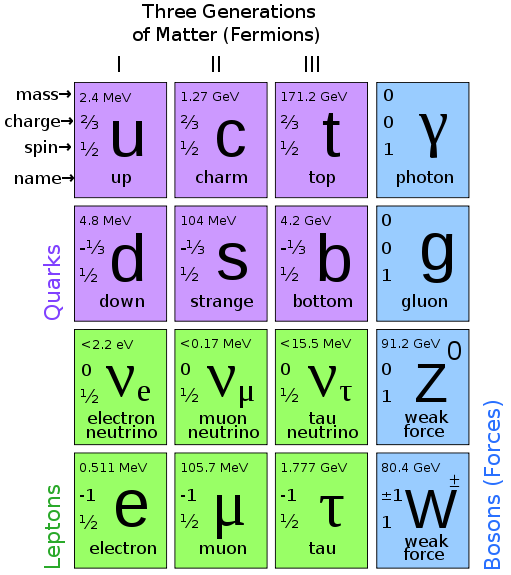
\includegraphics[width=0.6\textwidth]{imagens/standart_model.pdf}
\caption{O Modelo Padrão de partículas elementares. Extraído de
\cite{wiki_standart_model}.}
\label{fig:modelo_padrao}
\end{figure}

Além dessas partículas elementares, a Lei de Dirac prevê a
existência de uma anti-partícula para cada partícula carregada
com a mesma massa e rotação, mas cargas invertidas. A equação de Dirac para léptons neutrinos tambêm permite a existência de
anti-neutrinos. Quando um par de partícula e anti-partícula entram em contato
eles se aniquilam liberando sua energia de repouso $2mc$ em fótons e outras
partículas. Elas são representadas através de uma barra acima dos simbulos
das partículas, ou, no caso de partículas com indices de carga em seus símbulos, 
apenas os sinais da carga são modificados. A anti-partícula do elétron tem o nome de pósitron, por motivos
históricos \cite{Intro_Standard}. 

As forças são comunicadas através dos bóssoms, partículas elementares
transportadoras de campo. Cada força tem seu
bóssom característico: o glúon (g): força forte; o fóton $\gamma$: força
eletromagnética; e os bóssoms W e Z: força fraca. 
Os bóssoms W e Z possuem respectivamente massa de aproximadamente
80 e 90 GeV. Essa fato limita o alcance da força fraca a cerca $10^{-3}$ fm de,
uma vez que uma partícula de massa M só pode existir como parte de um estado
intermediário por tempo $\hbar/Mc^2$, viajando uma distância não maior que
$\hbar/Mc$. O bóssom W possui carga elétrica, enquanto o bóssom Z é neutro, sendo sua própria anti-partícula.
O glúon e o fóton não possuem carga, assim como massa de repouso, de forma que é esperado alcance de
interação infinito para os campos portados por essas partículas. 
Contudo, diferente do campo eletromagnético, o campo de
glúons é confinado a um alcance de 1 fm. 
Assim, para distâncias maiores a 1 fm, a força eletromagnética é dominante,
enquanto para distâncias menores, as interações forte e fraca também ocorrem.
Os físicos esperam adicionar a força gravitacional
através da partícula \emph{graviton}, que deverá ter rotação equivalente a 2
unidades de $\hbar$.
A intensidade relativa (em comparação com a interação forte) dos quatro tipos de
interações são mostradas na Tabela \ref{tab:interacoes}.

\begin{table}
\centering
\begin{tabular}{cc}
\hline
\textbf{Interação} & \textbf{Intensidade Relativa} \\
\hline
Forte & 1 \\
Eletromagnética & $10^{-2}$ \\
Fraca & $10^{-5}$ \\
Gravitacional & $10^{-39}$ \\
\hline
\label{tab:interacoes}
\end{tabular}
\caption{Intensidade Relativa (em comparação com a interação forte) dos diversos
tipos de interação. Extraído de \cite{tese_eduardo}.}
\end{table}

Duas leis de convervação muito importantes na Física de
Partículas são: Conjugação de Paridade e de Carga, referidas como Simetria CP. 
A Simetria CP diz que a física deve reagir
da mesma maneira se a partícula for alterada para sua anti-partícula (C) e refletida
espacialmente (P). Existem evidências que a Simetria CP é violada pela interação fraca \cite{Intro_Nuclear}.

Os léptons podem ser subdivididos em dois grupos, 
um com massa e carga elétrica idêntica unitária: elétron, múon e táon; 
e outro neutro em carga e massa reduzida, estando relacionados com os léptons
carregados: neutrino do elétron, neutrino do múon e neutrino do táon. Dos
léptons carregados, o múon e o táon só diferem dos elétrons na sua massa e no
seu tempo de vida finitos, sendo o elétron o único estável.
Experimentalmente observa-se que um lépton só pode mudar para outro do seu mesmo
subgrupo, assim como um lépton só pode ser criado ou destruido em conjunto com
um anti-lépton do mesmo subgrupo. Esse fato pode ser melhor observado no
decaimento descrito por \ref{eq:muon}, onde um múon decaí em um
elétron, lépton carregado, criando ao mesmo tempo um neutrino do múon e um
anti-neutrino do elétron, ambos do grupo de léptons neutrinos.
Nenhum dos léptons sofrem interações com os glúons, portadores da força forte.
No caso do subgrupo dos léptons neutrinos, eles tambêm não interagem com a força eletromagnética (fótons), 
uma vez que não têm carga, só interagindo com a força fraca e, por esse motivo,
são de difícil detecção \cite{Intro_Nuclear,Intro_Standard}.

\begin{equation} \label{eq:muon}
\mu^{-} \rightarrow \nu_{\mu} + e^- + \bar{\nu}_{e}
\end{equation}

Os quarks possuem tanto sabores, que lhes descreve as caracteristicas de massa e
carga elétrica, quanto um equivalente de carga de interação
forte, distinguido em três cores de carga forte: vermelho, verde e azul. 
Para cada geração existe um par de sabores, onde um dos constituintes do par tem
carga elétrica positiva, correspondente a $\frac{2e}{3}$,
e outro negativa, igual a $\frac{-e}{3}$. São os possíveis sabores: \emph{up}
(u) e \emph{down} (d), \emph{charm} (c) e \emph{strange} (s), \emph{top} (t) e
\emph{bottom} (b). 
Uma dificuldade da investigação experimental dos quarks é devida aos mesmos
nunca terem sidos observados isoladamente. Eles estão sempre confinados em sistemas
compostos, que se extendem a uma distância de até 1 fm, alcance máximo da
interação forte. Se da ao nome dos sistemas compostos por quarks e glúons de
hádrons, sendo os bárions e mésons os sistemas mais simples conhecidos. 
A Teoria da Cromodinâmica Quantica (QCD) prevê como os quarks e glúons 
interagem para formar os hádrons. Mesmo
em colisões de altas energias os quarks se agrupam rapidamente em hádrons,
formando jatos hadrônicos \cite{Intro_Nuclear}.
Os quarks sofrem influência de todas as forças descritas pelo Modelo Padrão.
 
Um largo espectro dos bárions podem ser explicados como uma cápsula contendo
três quarks confinados por glúons, sendo exemplos os prótons e neutróns. Os mésons, 
são compostos essencialmente por um quark e anti-quark ligados
transientemente por um glúon. Alguns dos mésons referidos neste trabalho são
os mésons mais leves existentes, os píons: $\pi^{+}$,
$\pi^{-}$ e $\pi^{0}$, compostos respectivamente por pares $u\bar{d}$, $\bar{u}d$ e
$u\bar{u}$ ou $d\bar{d}$, e os káons, os mais leves dos mésons estranhos
(contendo quarks $s$), $K^{+}$, $K^{0}$, $K^{0}_{S}$ e $K^{0}_{L}$, 
compostos pelos sistemas $u\bar{s}$, $d\bar{s}$,
$\frac{d\bar{s}+s\bar{d}}{\sqrt{2}}$, onde a diferença do $K^{0}_{S}$ e
$K^{0}_{L}$ está no tempo de vida médio dessas partículas. 
O próton ($uud$) é o único bárion estável, já o neutron ($udd$), apesar de estável na estrutura atômica,
quando isolado tem vida média de 15 minutos \cite{Intro_Standard}. Enquanto
isso, todos mésons são instáveis.
 
Outra simetria muito importante é conhecida como a Invariância de Gauge.
Ela prevê que todos os bóssoms de rotação unitária precisam ter
massa de repouso nula, se eles forem os únicos bóssoms da teoria.
Isso é aceitável para as teorias QED e QCD, uma vez que os
fótons e gluóns não possuem massa, mas é experimentalmente contraditório
para os bóssoms Z e W. A Invariância de Gauge tem um papel ainda mais forte
quando na teoria unificada eletrofraca, onde sua consequência é que todas as
partículas contêm massa nula. Foi introduzido um mecânismo, 
por Peter Higgs em 1964, para corrigir o Modelo Padrão de modo que ele atendesse
a essa formulação, conhecido como o bóssom de Higgs, portador do campo de Higgs. O bóssom de Higgs seria
uma partícula mediadora responsável de fornecer massa às partículas elementares.
A existência do bóssom de Higgs é a mais importânte previsão do Modelo Padrão
ainda não verificada experimentalmente e sua busca é de máxima importância para
a Física de Partículas. Diferente dos outros bóssoms, o
bóssom de Higgs teria rotação nula \cite{Intro_Nuclear}.

O progresso da ciência tem o comprometimento entre teoria e experimento. Kelvin
diz que sem medir ou poder expressar em números o assunto tratado, se há apenas
uma ideia inícial do conhecimento sobre o tema \cite{kelvin}. 
Na Física de Partículas Elementares, experimentos atualmente dependem
principalmente de grandes aceleradores de partículas. Outras fonte de avanços na
Física de Partículas são experimentos com raios cósmicos, estudados tantos
através de detectores na superficie terrestre como através de satelites 
\cite{nature_space_and_time}. 

De acordo com a Teoria da Relatividade, não há diferença qualitativa entre
massa e energia, essa é apenas quantitativa \cite{einstein} sendo descrita por
\ref{eq:einstein}, onde E é a energia, $m_0$ a massa de repouso, e c a constante que representa a
velocidade de propagação da luz no vácuo, aproximadamente $3\times 10^{8}$ m/s. Ao se acelerar
partículas de pequenas massas, é possível gerar partículas com maiores massas
através das interações ocorridas durante a colisão. Experimentos em
aceleradores de partículas tiveram seu início por volta de 1930, com o
acelerador linear \emph{Crockroft-Walton} em Cambridge, Reino Unido. Esse
acelerador atingia energias de 0.7 MeV com prótons. A tabela
\ref{tab:aceleradores} lista alguns dos aceleradores já construidos. Os
aceleradores podem ser lineares ou circulares, assim como de alvo fixo ou colisionadores
de feixes. Nos aceleradores de alvo fixo as partículas são aceleradas até
obterem a energia desejada e então direcionadas a um alvo estacionário. Já os
colisionadores de feixes, as partículas são aceleradas em feixes em direções
opostas e então colididas quando a energia desejada é atingida. A aceleração é
realizada através do uso de força eletrogmanética, de forma que apenas
partículas carregadas elétricamente são aceleradas.

\begin{equation} \label{eq:einstein}
E=m_0c^2
\end{equation}

\begin{table}
\centering
\begin{tabular}{lll}
\hline \hline \hline
\textbf{Máquina} & \textbf{Partículas Colididas} & \textbf{Início-Término} \\
\hline \hline
Tevatron & p: 900GeV & 1987 \\
(Fermilab, Batavia, Ilinóia) & $\bar{p}$: 900GeV & \\
\hline
SLC & $e^{+}$: 50GeV & 1989-1998 \\
(SLAC, Standford) & $e^{-}$: 50GeV & \\
\hline
HERA & e: 30GeV & 1992 \\
(DESY, Hamburgo) & p: 820GeV & \\
\hline
LEP2 & $e^{+}$: 81GeV & 1996-2000 \\
(CERN, Genebra) & $e^{-}$: 81GeV & \\
\hline
PEP-II & $e^{+}$: 9GeV & 1999-2008 \\
(SLAC, Standford) & $e^{-}$: 3.1GeV & \\
\hline
LHC & p: 7TeV & 2008 \\
(CERN, Genebra) & p: 7TeV & \\
\hline \hline
\label{tab:aceleradores}
\end{tabular}
\caption{Alguns aceleradores de partículas no mundo. Adaptado de \cite{Intro_Standard}.}
\end{table}

Muitos aceleradores de partículas utilizam prótons pois eles são mais facilmente
acelerados, atingindo níveis mais elevados de energia. Entretanto a
estrutura dos prótons são muito mais complexas (hádrons
compostos por quarks e glúons) que a dos elétrons (partícula elementar), de forma que as colisões com elétrons são 
de mais fácil compreensão. Como consquência, as
descobertas normalmente são realizadas através das colisões com prótons, enquanto as medições com
maior precisão são realizadas na colisão de elétrons \cite{nature_space_and_time}.
As colisões com íons de chumbo foram introduzidas em meados dos anos 80
para se estudar o Plasma de Quarks e Glúons (QGP) \cite{heavy_ions}.

O Modelo Padrão ainda deixa muitas questões em aberto. Não se foi capaz, até o
momento, de adicionar o campo gravitacional ao mesmo. São necessários a
determinação de cerca de 25 a 26 parâmetros quando considerando a existência do
bóssom de Higgs. Existem realmente tal ordem de parâmetros independentes na
natureza? Ainda, experimentos astronômicos mostram que apenas 4\% do universo é
composto pela materia conhecida no modelo padrão, outros 23\% são de matéria
escura, partículas ou conglomerados massivos que não brilham ou disseminam luz,
e os 73\% restantes, grande parte da energia do universo, são de energia escura,
totalmente desconhecida para a ciência atual. Indo mais além, o Modelo Padrão
não explica porque o universo se consiste quase totalmente por matéria e
praticamente nenhuma anti-matéria. Espera-se que o experimento LHC (seção
\ref{sec:lhc}) seja capaz de responder a essas perguntas, entre outras, 
e ajude os cientistas a resolverem as incoerências e problemas do modelo, quem sabe também reduzindo 
o número de parâmetros livres a serem determinados para um, ou dois.
\cite{nature_space_and_time,Intro_Nuclear}

\section{O Large Hadron Collider}
\label{sec:lhc}

Atualmente, o CERN está engajado no projeto LHC (Large Hadron
Collider), um acelerador de partículas circular de 27 quilômetros de
circunferência, situado no subsolo, dentre 50 e 175 m. 
No presente momento, ele realiza colisões de pacotes de prótons a uma energia
de 7 TeV no centro de massa, que serão expandidos a 14 TeV em 2013 \cite{webATLAS}.
O LHC apresenta uma oportunidade sem precedentes para conhecer os domínios da
nova física na região TeV e lançar luz sobre algumas das questões fundamentais
não resolvidas da Física das Partículas Elementares. 
Dentre os tópicos principais a serem testados pelo LHC estão \cite{hunt_for_physics}:

\begin{itemize}
\item \textbf{Busca pela Supersimetria (SUSY)}: Tida como uma provável base para o Modelo
Padrão\cite{Intro_Standard}. Algumas partículas previstas por esse modelo, as superpartículas, 
devem ser visualizada na região TeV;
\item \textbf{Busca pelo bóssom de Higgs}: Se tal partícula existir, o LHC deverá ser capaz de
observá-lo;
\item \textbf{Violação CP}: Estudo da violação da simetria-CP;
\item \textbf{Matéria escura}: Os candidatos mais relevantes vão além do Modelo
Padrão para descrever a matéria escura. Um dos possíveis modelos é a supergravidade;
\item \textbf{Física do quark \emph{top}}: Busca melhorar a compreensão da física dessa
partícula elementar, ainda não muito bem compreendida;
\item \textbf{Física do Z' (Z \emph{prime})}: Estudos dos possíveis bóssoms Z adicionais; 
\item \textbf{Assinaturas visiveis do Setor Escondido (HS)}: Modelo baseados em cordas
membranas provem um novo setor de física, o Setor Escondido, que poderá ser
explorado pelo LHC;
\item \textbf{Provar a origem da massa dos léptons neutrinos}: Se o mecânismo que gera
suas massas estiver na região TeV, o LHC poderá resolver essa questão;
\item \textbf{Caça por dimensões extras}: Modelo com ordens superiores de dimensões
oferecem alternativas para a Supersimetria;
\item \textbf{Busca por cordas no LHC}: A Teria de Cordas oferece a possibilidade de
união de todas as forças conhecidas na natureza, incluindo a gravidade. Muitos
trabalhos apresentados mostram predições de cordas na escala TeV.
\end{itemize}

Para desenvolver a altíssima energia necessária para o experimento, o CERN 
utiliza outros aceleradores construídos anteriormente, acelerando
sequencialmente os pacotes de prótons até atenderem
a energia desejada para a colisão. Na Figura \ref{fig:esquema_aceleradores} pode-se observar
o esquema de aceleração de prótons. Ele se inicia na extração de prótons de átomos
de hidrogeneo que são acelerados no LINAC 2, um acelerador linear,
que inicia a sequencia de aceleração. Em seguida são utilizados os aceleradores
circulares BOOSTER, PS, SPS, até finalmente abastecer o LHC com os pacotes de
prótons.

\begin{figure}[h!t]
\centering
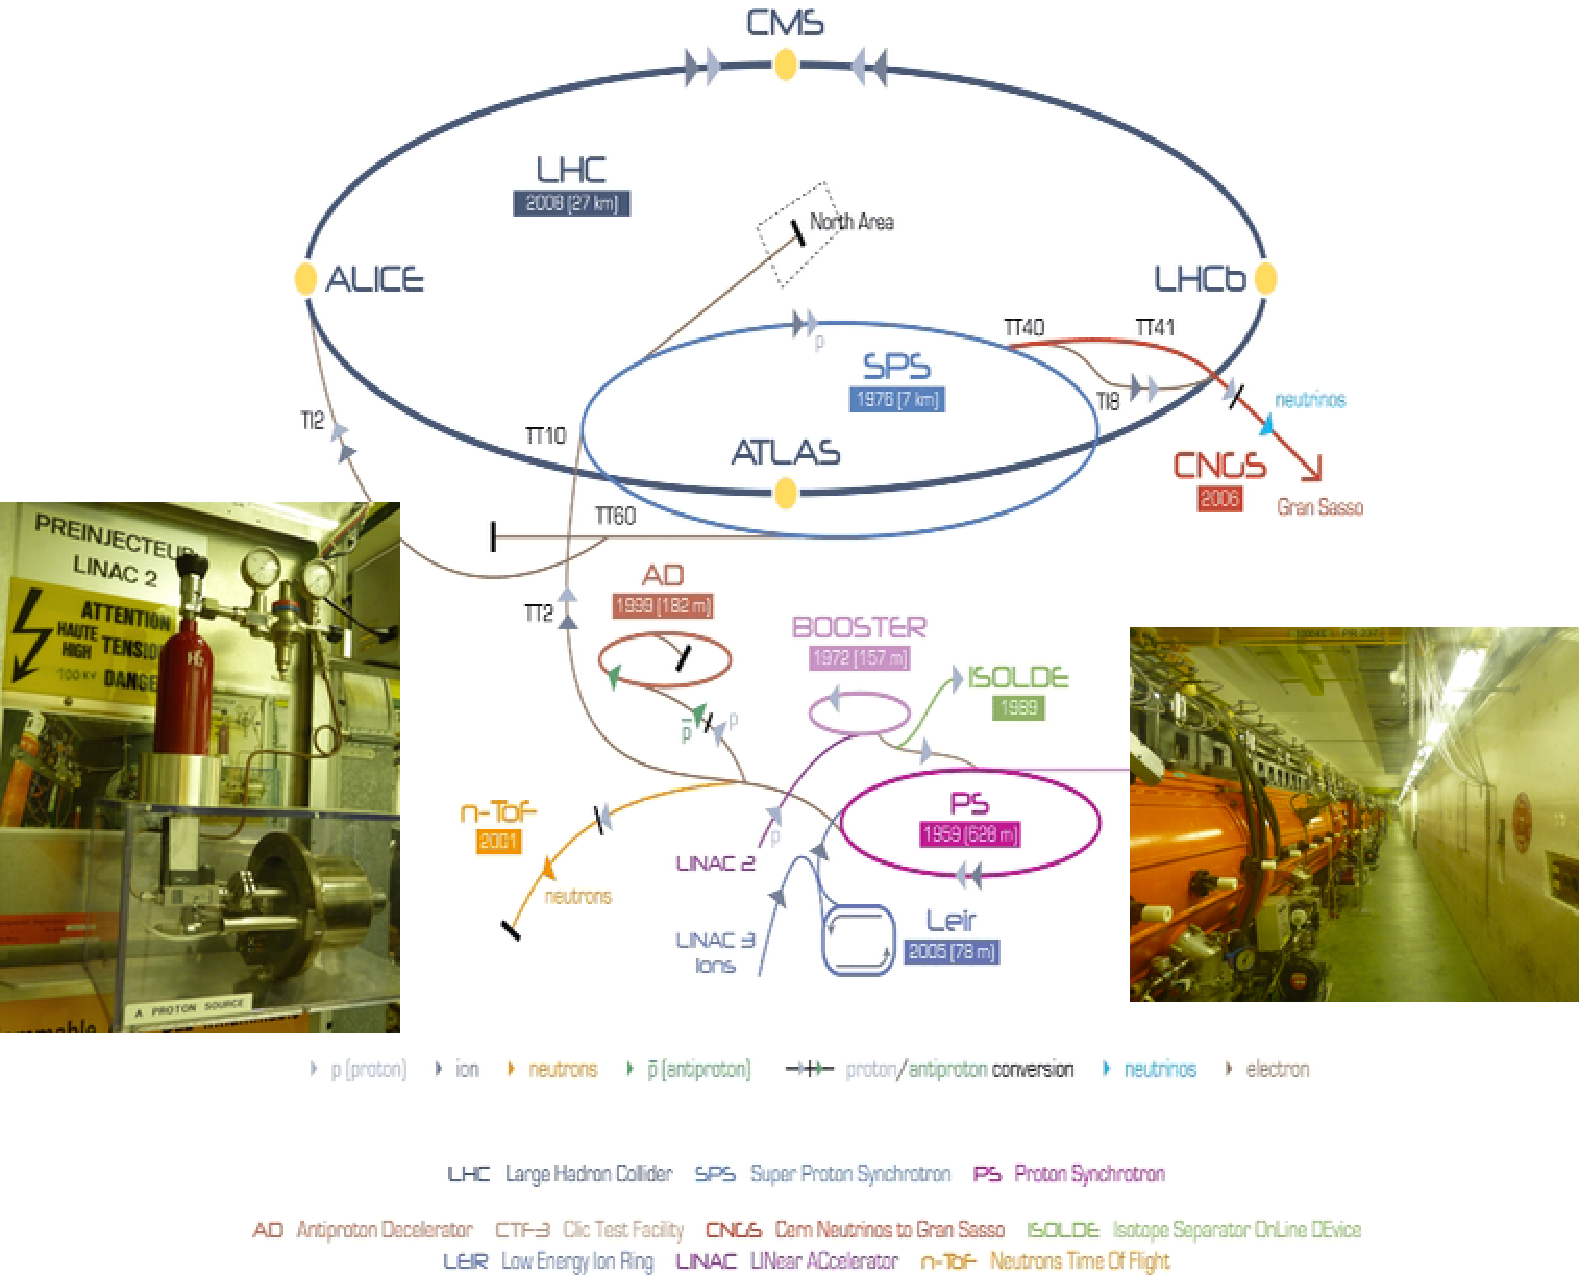
\includegraphics[width=\textwidth]{imagens/lhc_garrafa_linac2.pdf}
\caption{Os diferentes aceleradores e detectores do CERN, extraido de
\cite{cern_accelerators}. A seta cinza claro corresponde ao sentido do
deslocamento de prótons nos aceleradores. À esquerda, foto da garrafa
de onde são retirados os prótons, e na direita foto do LINAC 2.}
\label{fig:esquema_aceleradores}
\end{figure}

Tão importante quanto obter altas energias, é obter alta
luminosidade, um indicador da concentração 
de partículas no ponto de colisão, parâmetro similar a densidade de 
corrente $\overrightarrow{J}$ utilizado na engenharia elétrica. A luminosidade é definida por
\ref{eq:luminosidade}, onde a frequência de cruzamento entre feixes
\footnote{Traduzido do inglês \emph{bunch crossing rate}}, $f$, é de 40 MHz, $n$ é o número de feixes, 
$N_i$ equivale ao número de prótons em
cada pacote, correspondentes a $1.5\times10^{11}$ no início de uma
temporada\footnote{Traduzido do inglês \emph{run}} de colisão nominal, e,
finalmente, o termo A é a área dada pela secção transversal do feixe, 
de 64 microns (aproximadamente um fio de cabelo) no ponto de interação
\cite{webLHC}. No LHC, luminosidades de até $10^{34}cm^{-2}s^{-1}$ serão
atingidas.

\begin{equation} \label{eq:luminosidade}
L=fn\frac{N_1 N_2}{A}
\end{equation}

O número de colisões é diretamente proporcional a luminosidade, o que explica
se desejar elevadas luminosidades. A taxa de colisão é definida por
\ref{eq:taxa_colisao}, onde L é a luminosidade e $\sigma$ é a seção de choque,
expressa em mbarn. A seção de choque é de 110 mbarn para as colisões a 7 TeV, e
60 mbarn para a produção de colisões inelásticas.
Nesses valores se obtêm 19 eventos de colisões inelásticas para cada
cruzamento de feixes \cite{webLHC,ATLAS_TDR}.

\begin{equation}
R = L \times \sigma
\label{eq:taxa_colisao}
\end{equation}

Os eventos de colisões podem ser de dois tipos \cite{THESIS_LAR}:

\begin{enumerate}
\item \textbf{Colisões Rigidas}:
elas são devidas as interações de curto alcance,
resultando em grandes transferências de momemnto que produzindo partículas de
alto momento, assim como condições para a geração de novas partículas de altas
energias, como o bóssom de Higgs.
\item \textbf{Colisões Suaves}: 
é o tipo de iteração mais comum e devidas as interações de longo alcance entre dois prótons cruzantes. Os
resultados são partículas com grande momento longitudinal\footnote{Na direção de
propagação do feixe} e pouco momento transverso\footnote{Perpendicular à
propagação}. Esses eventos de colisão são
denominados de \emph{mininum bias} e são compostos na sua maioria por jatos.
\end{enumerate}

O experimento LHC conta com quatro detectores de maior escala: ATLAS, CMS, ALICE e
LHCb; e dois de menor escala: TOTEM e LHCf. O trabalho atual está definido no
escopo da colaboração do detector ATLAS (seção~\ref{sec:ATLAS}).

O ATLAS e o CMS são de propósito geral, ou seja, são capazes de estudar diversos
fenômenos físicos. O fato de existirem dois detectores projetados de forma
diferente, mas para o mesmo fim, é importante para que um possa confirmar o
resultado do outro.

O LHCb é um detector especializado no estudo do quark \textit{beauty} com o
intuito de investigar a diferença entre matéria e antimatéria.

O ALICE, por sua vez, estudará o QGP que será formado quando o
LHC fizer colisões de íons de chumbo.

Os dois menores detectores são o LHCf e o TOTEM. O LHCf, que se situa na mesma
caverna do ATLAS, estuda o comportamento de raios cósmicos, utilizando
partículas que não chegaram a colir no ponto de colisão, mas foram desviadas.
O TOTEM, que está instalado perto do CMS, estuda o feixe de prótons produzidos
pelo LHC, bem como a estrutura interna do próton.

\section{O Detector de Partículas ATLAS}
\label{sec:ATLAS}

O ATLAS (\textit{A Toroidal LHC Apparatus}) é o maior dos detectores que operam
no LHC, medindo 45 metros de comprimento e 25 metros de altura e largura. Como é
um detector de propósito geral, o detector registra dados sobre os eventos de
colisões de partículas que podem ser usados para estudos em diversas áreas da
física. 

O experimento está na fase de operação desde setembro de 2008 \cite{webLHCFirstBeam},
quando o primeiro feixe de partículas circulou no acelerador e os primeiros
eventos de colisão dos prótons com moléculas de gás dentro do tubo do acelerador
foram registrados. Para coletar dados suficientes para as análises físicas o
experimento pode durar cerca de 20 anos \cite{ATLAS_TDR}.

O ATLAS foi construído e é operado por uma colaboração internacional envolvendo
cerca de 2500 físicos de mais de 174 instituições e laboratórios de 38 países
\cite{webATLAS}. Esses números incluem a UFRJ, que participa através da COPPE,
da Escola Politécnica e do Instituto de Física. O detector é composto por 4
sub-detectores: o Inner detector, detector de traço; o Liquid Argon, que é o
calorímetro eletromagnético; o Tile Calorimeter, que é o calorímetro hadrônico,
e o Muon Spectrometer responsável por realizar medições sobre os múons. Cada uma
dessas partes teve seus componentes construídos por um grupo diferente,
pertencente às instituições colaboradoras.  Uma vez construídos e testados, os
componentes foram levados ao CERN, onde foram instalados em seus lugares
definitivos. Para coordenar essa montagem e fornecer a infra-estrutura
necessária no local do experimento, existe o grupo da Coordenação Técnica
({\it ATLAS Technical Coordination}).

\subsection{O Sistema de Calorimetria do ATLAS}
\label{ssec:calorimetria}


\section{Ferramentas Utilizadas na Colaboração}
\label{sec:ferramentas}

